% !TeX root = Report.tex
\section{Results}

\subsection{Methodology}

In our simulations we tested networks of various sizes (15, 30 and 48 nodes) aligned in a grid. The nodes were placed such that every node had four neighbours, one to the north, south, east and west, except for nodes in the edge which had three neighbours and the nodes in the corner that had two neighbours. The sink was always placed in the top left corner and was always assigned the address ``1.0''. The predicate checking algorithm was started as soon as the nodes had come online, the nodes then waited for 5 minutes to allow the predicate checking algorithm time to setup and then the TDMA algorithm was started. The simulation was run for 35 minutes overall and then it was terminated. After the predicate checking algorithm had setup, the predicate was checked every 2 or 4 minutes depending on the parametrisation. When setting up the Cooja simulator to run the simulations the radio medium was set to be ``UDGM: Distance Loss'', the mote startup delay was set to be 1000ms and a random seed was set to be used on every reload.

To gather metrics on the energy usage of the motes, a Contiki library called rimestats\footnote{\url{http://contiki.sourceforge.net/docs/2.6/a00357\_source.html}} was used. This library is built into the MAC layer and records deep statistics, we simply used the sent and received message counts. Contiki comes with a library to estimate the energy usage \cite{Dunkels:2007:SOE:1278972.1278979}, however, we wish to keep things simple and focus on the number of messages being sent and received.

In order to calculate how many messages the TDMA algorithm involved we implemented our own sent and received counters that were incremented when a message was sent or received. As the TDMA protocol was implemented with simple broadcasts there is a one-to-one correspondence between the number of successful broadcasts and the number of transmissions done at the MAC layer, the same is also true for receiving a message. To calculate the message cost of the predicate evaluation algorithm, the difference between the total and the TDMA messages was taken.

To check that a predicate was successfully evaluated the TDMA algorithm printed any changes in the assigned slot as well as the time the slot was changed. When a predicate was evaluated on a node the time it was evaluated as well as the result was printed. Analysis scripts then evaluated the predicate using the most recent slot value from before or up to when the predicate was evaluated to evaluate the predicate itself. This result was then compared with the actual result of the predicate. The results were compared whether or not the predicate response message reached the sink.

We ran these experiments using two different predicates, one that required 1-hop information and one that required 2-hop information. Both were checking to see if there were slot collisions and were the same two predicate that were mentioned as examples in \autoref{sec:example-predicates}. Below the code and logic for the two predicates is reproduced.

\begin{figure}[H]
\begin{minipage}{.5\linewidth}
\begin{lstlisting}[language=Hoppy]
[all]
function 1 as slot returning int in
    using Neighbours(2) as twohopn in
        @(x : twohopn ~
            slot(x) != slot(this)
        )
\end{lstlisting}
\end{minipage}%
\begin{minipage}{.5\linewidth}
\begin{align*}
&				\forall n \in \text{Nodes} \cdot \\
& \hspace{2em}		\forall n' \in \text{Neighbours}(n, 2) \cdot \\
& \hspace{4em}				\text{slot}(n) \neq \text{slot}(n')
\end{align*}
\end{minipage}
\vspace{-1em}
\caption{Check that no two neighbours have the same slot (2-hop information)}
\label{fig:two-hop-slot-pred-lang-results}
\end{figure}
\vspace{-2em}
\begin{figure}[H]
\begin{minipage}{.5\linewidth}
\begin{lstlisting}[language=Hoppy]
[all]
function 0 as addr returning int in
function 1 as slot returning int in
    using Neighbours(1) as onehopn in
        @(a : onehopn ~
            @(b : onehopn ~ addr(a) != addr(b)
                => slot(a) != slot(b))
             & slot(a) != slot(this)
        )
\end{lstlisting}
\end{minipage}%
\begin{minipage}{.5\linewidth}
\begin{align*}
&				\forall n \in \text{Nodes} \cdot \\
& \hspace{2em}		\forall n' \in \text{Neighbours}(n, 1) \cup \{n\} \cdot \\
& \hspace{4em}			\forall n'' \in \text{Neighbours}(n, 1) \cup \{n\} \cdot \\
& \hspace{6em}				\text{addr}(n') \not= \text{addr}(n'') \\
& \hspace{8em}					\implies \text{slot}(n') \neq \text{slot}(n'')
\end{align*}
\end{minipage}
\vspace{-1em}
\caption{Check that no two neighbours have the same slot (1-hop information)}
\label{fig:one-hop-slot-pred-lang-results}
\end{figure}

\subsection{Analysis}

\begin{figure}[H]
\centering
\subfigure[Rx]{%
	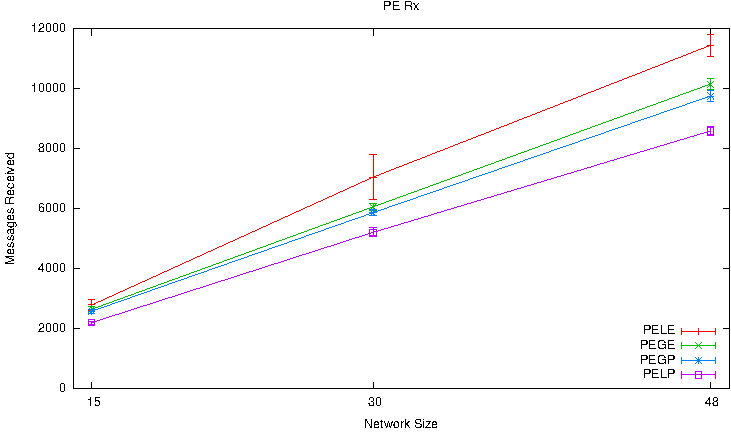
\includegraphics[width=0.44\linewidth]{../Results/Graphs/4.0/1HOP/messagesPE/rx/graph.pdf}
	\label{fig:predeval4.0-rx}
}
\subfigure[Tx]{%
	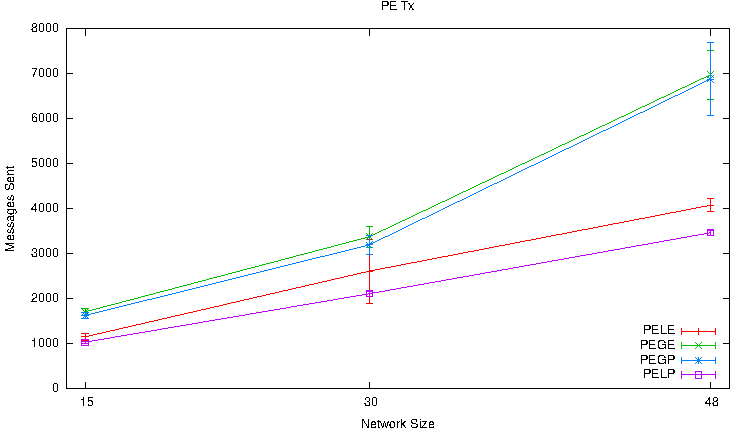
\includegraphics[width=0.44\linewidth]{../Results/Graphs/4.0/1HOP/messagesPE/tx/graph.pdf}
	\label{fig:predeval4.0-tx}
}

\subfigure[Percentage of  predicates correctly evaluated]{%
	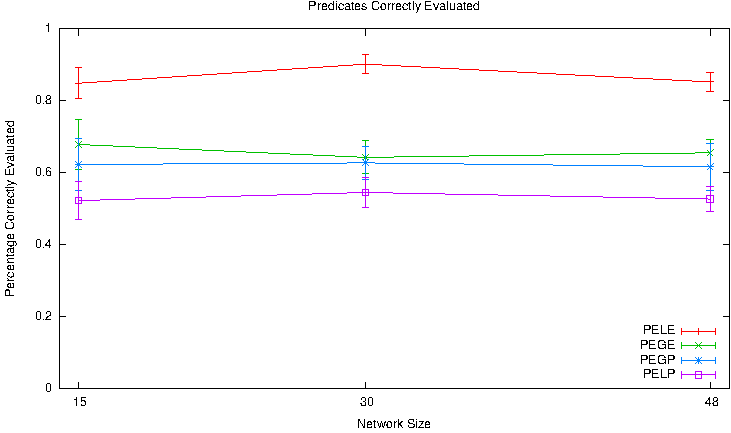
\includegraphics[width=0.44\linewidth]{../Results/Graphs/4.0/1HOP/pcCorrectlyEvaluated/graph.pdf}
	\label{fig:predeval4.0-correct}
}
\subfigure[Percentage of responses received]{%
	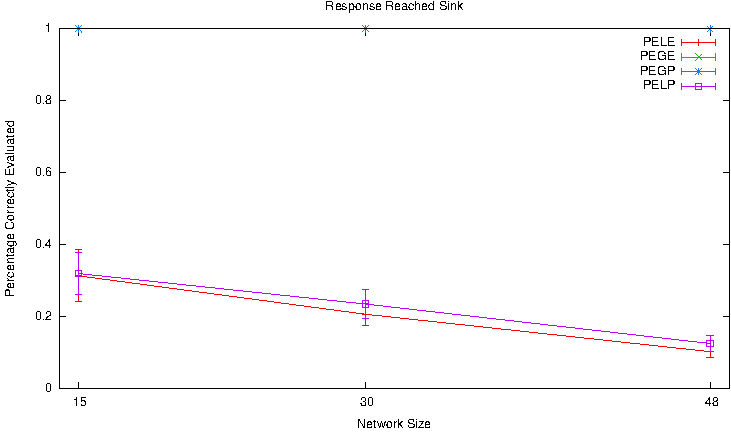
\includegraphics[width=0.44\linewidth]{../Results/Graphs/4.0/1HOP/pcResponsesReachedSink/graph.pdf}
	\label{fig:predeval4.0-recv}
}
\caption{Results when predicate period is every 4.0 minutes using a 1-hop predicate}
\label{fig:predeval4.0}
\end{figure}

The first point of note from the data presented in \autoref{fig:predeval4.0} is that in \subref{fig:predeval4.0-recv}, both of the global predicate evaluation algorithms (PEGE and PEGP) show a 100\% delivery rate. While this may initially appear very impressive, this simply arises from the facts that these predicates are evaluated at the sink, and that the graph shows the receipt of evaluated predicates sent from the evaluation location to the sink -- as no messages need to be sent, it is vacuously true that no messages will fail to arrive. The two local predicate checking algorithms, however, showed a more predictable trend of successfully delivering fewer responses as the network size increased, though the specific values of these rates are disappointingly low. The values suggest that only nodes in the immediate neighbourhood of the sink are being successful in sending the results of their predicate evaluations. As the network grows in size, the proportion of nodes within this range of the sink decreases, resulting in the trend shown. We believe that this result is due to the way the mesh protocol provided by Contiki works, as it first needs to flood the network with a route discovery message and then waits for a route reply from the target node. However, due to the high amount of traffic it is likely that either or both of these messages are simply being lost. A solution to this would be to have a setup phase, during which every node discovers their respective paths to the sink, before predicate evaluation (or any other main algorithm that is being executed) begins.

Graph \subref{fig:predeval4.0-correct}, showing the rate of correct predicate evaluation, reveals much more useful information: locally-evaluated event-triggered predicates (PELE) show significantly higher accuracy than each of the other algorithms. Global event-based predicates (PEGE) were shown to have the second-highest accuracy, though this accuracy was only slightly higher than that of the periodic counterpart so it cannot be concluded that an event-based approach is universally better (within the scope of this metric). There may be a connection between PELE having the highest number of received messages (graph \subref{fig:predeval4.0-rx}) and its superior accuracy in evaluation; the premise being that more messages being received could give a node more data to use when evaluating a given predicate, in turn making it more likely to return a correct response. This notion of higher message delivery rates for PELE is somewhat corroborated by the number of transmissions shown in \subref{fig:predeval4.0-tx} -- PELE is responsible for the second lowest number messages sent. However, the cause of PELE alone having a significantly higher success rate in delivering messages is as yet unknown, so more definitive information on this front would require further scrutiny using testing methods that may well prove infeasible in a resource-constrained system.

It is also good to note that as the network size increases the correctness of predicate evaluation remains effectively constant, with only small fluctuations. From this we can say that the predicate evaluation libraries are highly scalable with respect to the size of the network and the accurate evaluation of the predicate. However, as has been mentioned before they scale poorly with respect to the number of responses the reach the sink.

As messages sent and received use the most energy in a WSN system \cite{Shnayder04} we will use message transmit and receive statistics to evaluate the energy usage of the algorithms. In graphs \subref{fig:predeval4.0-rx} and \subref{fig:predeval4.0-tx}, local periodic predicate evaluation is the most conservative, however it also shows the lowest accuracy for its evaluations so these results show little in the way of benefits to using this algorithm. By contrast, the most accurate algorithm, PELE, has a higher (yet still moderate) level of energy consumption. An important observation is that the energy demands of global predicate evaluation -- both of which showed middling accuracy -- increase faster than those of local evaluation as network size increases. This is because global evaluation requires data from the entire network, and the operating of the mesh routing protocol means that nodes lying further from the sink will have to have their messages forwarded by a greater number of intermediate nodes, giving exponential growth in the number of messages sent. The local evaluation algorithms show a more linear trend as the size of a node's 1- or 2-hop neighbourhood may not increase due to the presence of more nodes in the network -- all that is guaranteed is that there will be more such neighbourhoods in which to evaluate predicates.

\begin{figure}[H]
\centering
\subfigure[Rx]{%
	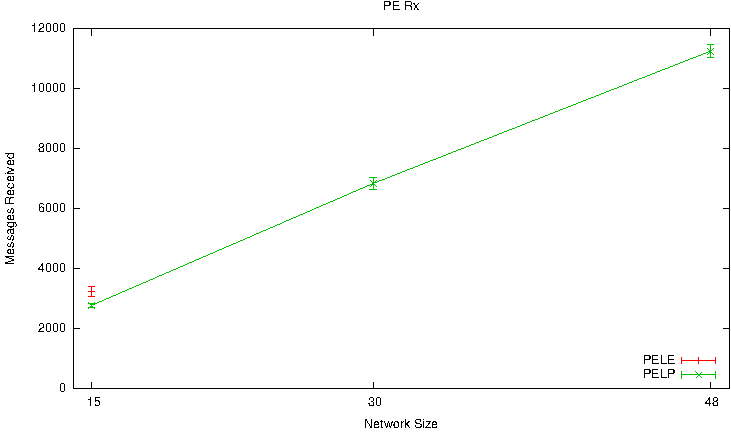
\includegraphics[width=0.44\linewidth]{../Results/Graphs/2.0/1HOP/messagesPE/rx/graph.pdf}
	\label{fig:predeval2.0-rx}
}
\subfigure[Tx]{%
	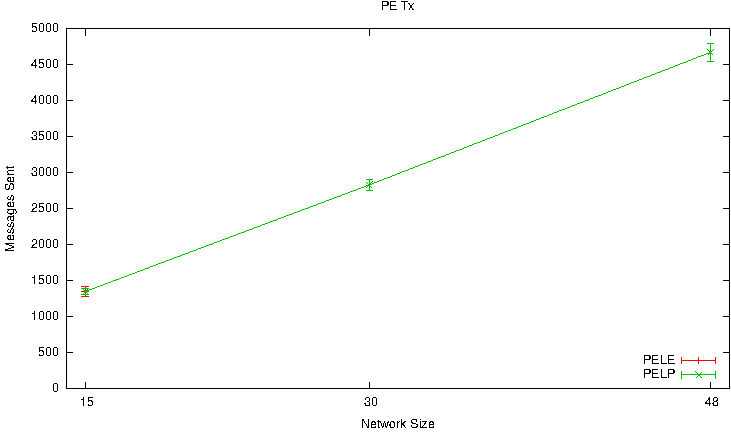
\includegraphics[width=0.44\linewidth]{../Results/Graphs/2.0/1HOP/messagesPE/tx/graph.pdf}
	\label{fig:predeval2.0-tx}
}

\subfigure[Percentage of predicates correctly evaluated]{%
	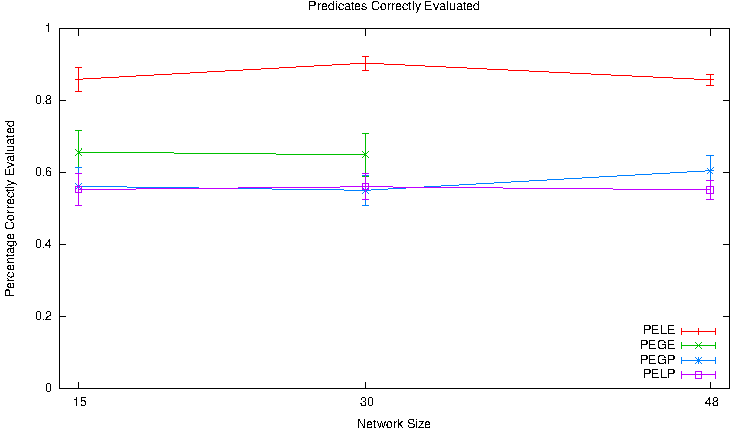
\includegraphics[width=0.44\linewidth]{../Results/Graphs/2.0/1HOP/pcCorrectlyEvaluated/graph.pdf}
	\label{fig:predeval2.0-correct}
}
\subfigure[Percentage of responses received]{%
	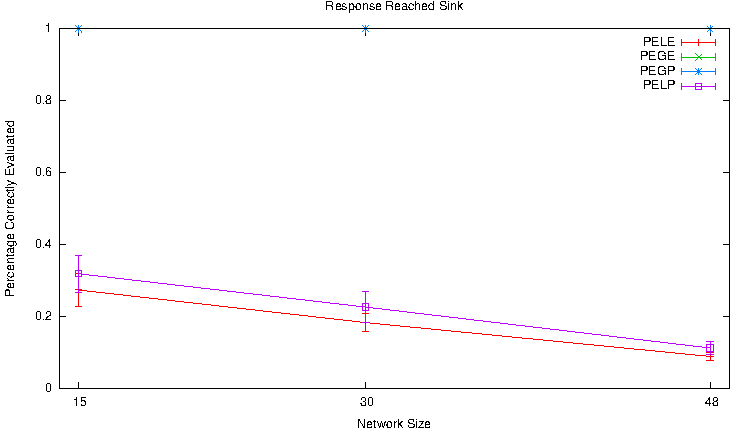
\includegraphics[width=0.44\linewidth]{../Results/Graphs/2.0/1HOP/pcResponsesReachedSink/graph.pdf}
	\label{fig:predeval2.0-recv}
}
\caption{Results when predicate period is every 2.0 minutes using a 1-hop predicate}
\label{fig:predeval2.0}
\end{figure}

At first glance of figure \autoref{fig:predeval2.0} the results seem to mirror those of figure \autoref{fig:predeval4.0}, however there is a key difference, in that the performance of the global periodic-based implementation had a lower success rate, when the predicate period is 2.0 minutes. This is likely due to the fact that messages are sent more often, but the delays in the aggregation tree remains the same. Therefore, it is likely that the aggregation tree affected how the predicates are evaluated by limiting how fast data from the edges of the network can reach the base station for evaluation. It is possible that the aggregation tree could be tweaked to decrease its wait period before sending messages onwards to increase the accuracy of evaluation, however, this would likely increase energy usage further.

The graphs also show that there were a larger number of messages both sent and received in these tests (figures \autoref{fig:predeval2.0-rx} and \autoref{fig:predeval2.0-tx}), although this can be attributed to the fact the predicate period is more often, requiring more messages to be passed around the network. Comparing the two sets of data we can see there were similar performance levels, regardless of the predicate period length. It can also be suggested that increasing the predicate period would increase the evaluation success rate, as there would be fewer collisions of messages in the network. Of course, based on the above reasoning, increasing the period would also decrease the number of messages sent by the periodic implementations and would thus extend battery life.

\begin{figure}[H]
\centering
\subfigure[Rx]{%
	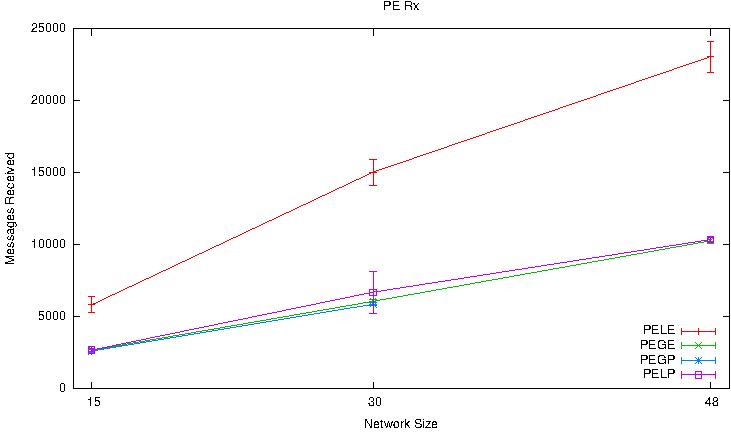
\includegraphics[width=0.44\linewidth]{../Results/Graphs/4.0/2HOP/messagesPE/rx/graph.pdf}
	\label{fig:predeval2hop-rx}
}
\subfigure[Tx]{%
	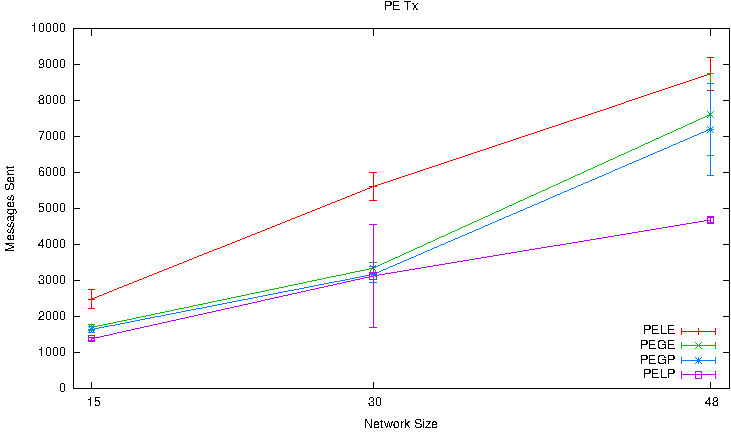
\includegraphics[width=0.44\linewidth]{../Results/Graphs/4.0/2HOP/messagesPE/tx/graph.pdf}
	\label{fig:predeval2hop-tx}
}

\subfigure[Percentage of predicates correctly evaluated]{%
	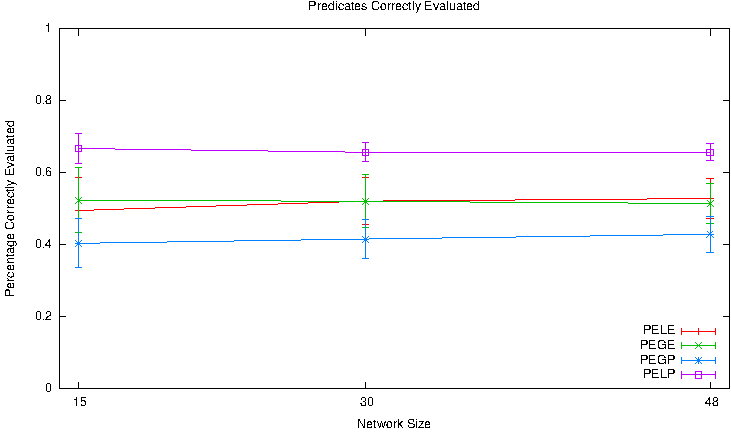
\includegraphics[width=0.44\linewidth]{../Results/Graphs/4.0/2HOP/pcCorrectlyEvaluated/graph.pdf}
	\label{fig:predeval2hop-correct}
}
\subfigure[Percentage of responses received]{%
	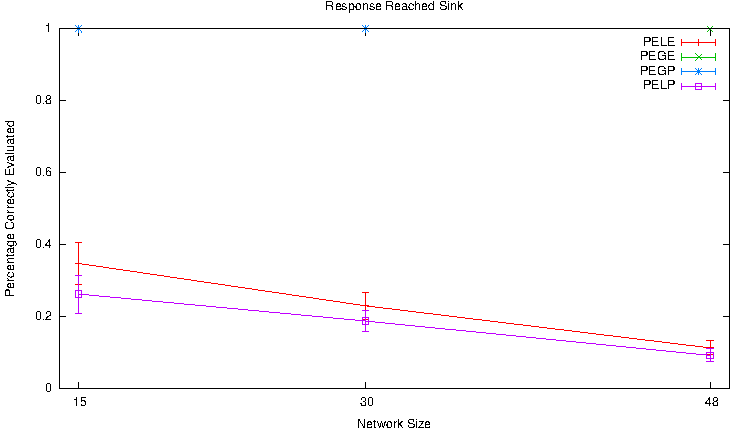
\includegraphics[width=0.44\linewidth]{../Results/Graphs/4.0/2HOP/pcResponsesReachedSink/graph.pdf}
	\label{fig:predeval2hop-recv}
}
\caption{Results when predicate period is every 4.0 minutes using a 2-hop predicate}
\label{fig:predeval-2hop-4.0}
\label{fig:predeval2hop}
\end{figure}

The previous two sets of results in \autoref{fig:predeval4.0} and \autoref{fig:predeval2.0} were for the 1-hop variant of the TDMA slot collision predicate. In \autoref{fig:predeval-2hop-4.0} results for the alternative 2-hop predicate are shown. There are a number of patterns that differ and some that remain the same.

To begin with we observe the same behaviour with respect to the delivery ratio of failure response messages in Figure \autoref{fig:predeval2hop-recv}. Predicates that are evaluated at the root node of the tree continue to have a 100\% delivery rate, while nodes evaluating in-network continue to have poor delivery rates that decrease in larger networks. The issue here is the same as the problem encountered with the 1-hop predicate results, so the same solution proposed would apply here.

Next, we have very different patterns of number of messages sent in Figure \autoref{fig:predeval2hop-tx}. We find that PELE requires the largest number of transmissions and PELP requires the fewest, with both growing linearly with respect to network size, whereas the global predicate evaluators use energy between these two levels and there number of transmissions increase faster than linearly. The difference here is that it is no longer the case that global evaluators require the most number of message to be sent. In fact the global evaluators use almost the same number of messages when comparing the 2-hop predicate results to the 1-hop predicate results. This is because the structure of sending messages to a node for predicate evaluation is the same in both 1-hop and 2-hop predicate evaluation, it is via an aggregation tree. The local in-network predicates are where large increases in messages sent occur. These increases are down to the fact that the neighbourhood of information that needs to be disseminated has increased from 1-hop to 2-hops. We see that this affects PELE more than it does PELP, for example for size 15 networks both local predicate evaluators transmit about 1000 message when evaluating the 1-hop predicate, whereas when evaluating the 2-hop predicate PELP sends about 1500 messages and PELE sends 2500 messages. So it when increasing the size of data that needs to be requested our event-based predicate evaluator will send more messages.

There is also a very interesting difference with respect to the correctness of predicate evaluation. When evaluating the 1-hop predicate the local in-network event-based evaluator performed best. However, for the 2-hop the local periodic evaluator performed best, we would expect that usually this would have been caused by the increase in message transmissions leading to a busier network with more collisions and message lost. Except that as the network size increases the number of messages transmitted increases, but the percentage of predicates that were correctly evaluated remains the same, so it would initially appear that collisions do not factor in. On the other hand, because these predicates are evaluated in-network they are by definition local, so increases in messages transmitted across the whole network may not paint an accurate picture. What we believe to be the case is that, compared to the 1-hop predicate, the 2-hop predicate has more local traffic and thus more local collisions which lead to event-based in-network evaluators to perform badly as lots of redundant data is transmitted. However, with in-network periodic evaluators data is only transmitted when it is asked for. So while event-based data sending may have helped for 1-hop predicates with respect to the greater number of transmissions, due to the increased number of hops data needs to travel to evaluate 2-hop predicate sending data when it changes actually leads to more local collisions leading to less current data reaching nodes, causing event-based evaluators to perform worse for 2-hop predicates than 1-hop predicates.

Another point is that for 2-hop evaluation the percentage of predicates correctly evaluated is generally lower than when evaluating 1-hop predicates. This is likely caused by the fact that more data is required, so there is a greater chance for more of it to be out-of-date by the time it reaches the evaluating node. There is also a greater chance for not all the data to reach the node evaluating the predicate (as there is simply more data being transmitted). Either of these two issues could have lead to the overall decrease in accuracy of evaluating the predicate.

\subsection{Conclusion}

To conclude it appears that deciding on which implementation to use when evaluating predicates depends on the size of the network and the predicate being evaluated. For predicates that involve no neighbour information or 1-hop neighbour information, evaluating them in network using PELE or PELP is preferred. PELE should most likely be used if data changes infrequently. We predict there will come a point where periodic sending of data will be better as the excess messages generated by frequent changes will lead to higher energy usage and more collisions (lower successful evaluations).

For predicates that use 2-hop information it would appear that using PELP is preferable due to the lower energy usage and high chance of a successful evaluation. We predict that as the size of the neighbour information increases, it will become more preferable to use global predicate evaluators.

For small networks there seems to be little difference between local and global predicate evaluators. However, as the network size increases it becomes less viable to use global evaluators due to the increase in energy.

So overall, deciding on where to evaluate a predicate is still a non-obvious decision. It depends on many factors, and these solutions still have the potential to be further optimised towards certain criteria.

